\section*{Questão 2: Convergência de passeios aleatórios}
Considere um passeio aleatório preguiçoso (com $p = 1/2$) caminhando sobre um grafo com $n$ vértices. Estamos interessados em entender a convergência da distribuição $\pi(t)$ em diferentes grafos. Assuma que o passeio sempre inicia sua caminhada no vértice $1$, ou seja, $\pi_1(0) = 1$. Considere os seguintes grafos: grafo em anel ($n = 125$), árvore binária cheia ($n = 127$), grafo em reticulado (grid) com duas dimensões ($n = 121$).

\begin{enumerate}
    \item Para cada grafo, construa a matriz de transição de probabilidade (ou seja, determine $P_{ij}$ para todo vértice $i, j$ do grafo). Atenção com a numeração dos vértices!
    \begin{resposta}
        Independente do grafo, a matriz de transição de probabilidade $P$ é dada por:
        $$
            P_{ij} = \begin{cases}
                1/2 & \text{se } i = j \\
                1/2d_i & \text{se } [i \neq j] \land [(i,j) \in E] \\
                0 & \text{caso contrário}
            \end{cases}
        $$
        onde $d_i$ é o grau do vértice $i$ e $E$ é o conjunto de arestas do grafo, ou seja, pares $(i,j)$ que representam arestas entre os vértices $i$ e $j$, se a aresta existir.

        \begin{itemize}
            \item Grafo em anel ($n = 125$):
            $$d_i = 2 \quad \forall i \in \{1, \dots, 125\}$$
            $$
            P_{ij} = \begin{cases}
                1/2 & \text{se } i = j \\
                1/4 & \text{se } [i \neq j] \land [(i,j) \in E] \\
                0 & \text{caso contrário}
            \end{cases}
            $$
            \item Grafo em árvore binária cheia ($n = 127$):
            
            Começando a numeração do nó raiz como $1$, temos:
            $$ 2 i \leq 127 \quad \Rightarrow \quad i \leq 63.5 $$
            Isso significa que os nós $i \in \{2,\dots,63\}$ são nós internos, enquanto os nós $i \in [64, 127]$ são folhas. Assim, temos:
            $$d_i = \begin{cases}         
                2 & \text{se } i \text{ é raiz }  (i=1)\\
                3 & \text{se } i \text{ é nó interno } (i \in \{2,\dots,63\}) \\
                1 & \text{se } i \text{ é folha } (i \in \{64,\dots,127\}) \\
            \end{cases}$$
            $$
            P_{ij} = \begin{cases}
                1/2 & \text{se } i = j \\
                1/4 & \text{se } [i \neq j] \land [(i,j) \in E] \land [i=1] \quad \text{(raiz)} \\
                1/6 & \text{se } [i \neq j] \land [(i,j) \in E] \land [i \in \{2,\dots,63\}] \quad \text{(nós internos)} \\
                1/2 & \text{se } [i \neq j] \land [(i,j) \in E] \land [i \in \{64,\dots,127\}] \quad \text{(folhas)} \\
                0 & \text{caso contrário}
            \end{cases}
            $$

            \item Grafo em reticulado (grid) com duas dimensões ($n = 121$):
            
            Numerando os vétices de forma crescente da esquerda para a direita e de cima para baixo, temos:
            $$d_i = \begin{cases}         
                2 & \text{se } i \in \{1, 11, 111, 121\} \quad \text{(cantos)} \\
                3 & \text{se } 
                    \begin{cases}
                        & i \in \{2,\dots,10\} \quad \text{(borda de cima)} \\
                        & i \in \{112,\dots,120\} \quad \text{(borda de baixo)} \\
                        & i \in \{12, 23, 34, 45, 56, 67, 78, 89, 100\} \quad \text{(borda da esquerda)} \\
                        & i \in \{22, 33, 44, 55, 66, 77, 88, 99, 110\} \quad \text{(borda da direita)}
                    \end{cases} \\
                4 & \text{caso contrário (nós internos)}
            \end{cases}
            $$

            $$
            P_{ij} = \begin{cases}
                1/2 & \text{se } i = j \\
                1/4 & \text{se } i \neq j \text{, } (i,j) \in E \text{ e }i \text{ é canto} \\
                1/6 & \text{se } i \neq j \text{, } (i,j) \in E \text{ e }i \text{ é borda} \\
                1/8 & \text{se } i \neq j \text{, } (i,j) \in E \text{ e }i \text{ é nó interno} \\
                0 & \text{caso contrário}
            \end{cases}
            $$
        \end{itemize}
    \end{resposta}

    \item Determine analiticamente a distribuição estacionária para cada grafo (ou seja, determine $\pi_i$ para cada vértice $i$ do grafo).
    \begin{resposta}
        Independente do grafo (dentre os 3 do enunciado), a matriz de transição de probabilidade $P$ do passeio preguiçoso é dada por:
        $$
        P = \frac{1}{2}I + \frac{1}{2}P',
        $$
        onde o termo $\frac{1}{2}I$ representa a probabilidade de permanecer no mesmo vértice, e o termo $\frac{1}{2}P'$ representa a probabilidade de transitar para um vértice vizinho.
        
        A equação de equilíbrio estacionário fica:
        $$
        \pi = \pi P = \pi \left( \frac{1}{2}I + \frac{1}{2}P' \right) = \frac{1}{2}\pi + \frac{1}{2}\pi P'.
        $$
        
        Subtraindo $\frac{1}{2}\pi$ de ambos os lados:
        $$
        \frac{1}{2}\pi = \frac{1}{2}\pi P' \Rightarrow \pi = \pi P'.
        $$
        
        Ou seja, o \textit{self-loop} introduzido pelo passeio preguiçoso não altera a distribuição estacionária. Basta, portanto, calcular a distribuição estacionária do passeio aleatório padrão, com matriz de transição $P'$.
        
        Para o passeio aleatório padrão, a distribuição estacionária é dada por:
        $$\pi_i = \frac{d_i}{K}, \text{ onde } K=\sum_i d_i=2m \text{, sendo } m \text{ o número de arestas do grafo.} $$

        \begin{itemize}
            \item Grafo em anel ($n = 125$):
            $$d_i = 2 \quad \forall i \in \{1, \dots, 125\}$$
            $$ m = 125 $$
            $$ \pi_i = \frac{2}{2 \cdot 125} = \frac{1}{125} \quad \forall i \in \{1, \dots, 125\} $$

            \item Grafo em árvore binária cheia ($n = 127$):
            $$d_i = \begin{cases}         
                2 & \text{se } i \text{ é raiz }  (i=1)\\
                3 & \text{se } i \text{ é nó interno } (i \in \{2,\dots,63\}) \\
                1 & \text{se } i \text{ é folha } (i \in \{64,\dots,127\}) \\
            \end{cases}$$
            $$ m = 127 - 1 = 126 $$
            $$\pi_i = \begin{cases}         
                \frac{2}{2 \cdot 126}=\frac{1}{126} & \text{se } i \text{ é raiz }  (i=1)\\
                \frac{3}{2 \cdot 126}=\frac{1}{84} & \text{se } i \text{ é nó interno } (i \in \{2,\dots,63\}) \\
                \frac{1}{2 \cdot 126}=\frac{1}{252} & \text{se } i \text{ é folha } (i \in \{64,\dots,127\}) \\
            \end{cases}$$

            \item Grafo em reticulado (grid) com duas dimensões ($n = 121$):
            $$d_i = \begin{cases}         
                2 & \text{se } i \in \{1, 11, 111, 121\} \quad \text{(cantos)} \\
                3 & \text{se } 
                    \begin{cases}
                        & i \in \{2,\dots,10\} \quad \text{(borda de cima)} \\
                        & i \in \{112,\dots,120\} \quad \text{(borda de baixo)} \\
                        & i \in \{12, 23, 34, 45, 56, 67, 78, 89, 100\} \quad \text{(borda da esquerda)} \\
                        & i \in \{22, 33, 44, 55, 66, 77, 88, 99, 110\} \quad \text{(borda da direita)}
                    \end{cases} \\
                4 & \text{caso contrário (nós internos)}
            \end{cases}
            $$
            $$ m_1 = 10 \cdot 11 = 110 \quad \text{(conexões verticais)}$$
            $$ m_2 = 10 \cdot 11 = 110 \quad \text{(conexões horizontais)}$$
            $$ m = m_1 + m_2 = 110 + 110 = 220 $$
            $$\pi_i = \begin{cases}         
                \frac{2}{2 \cdot 220} = \frac{1}{220} & \text{se } i \in \{1, 11, 111, 121\} \quad \text{(cantos)} \\
                \frac{3}{2 \cdot 220} = \frac{3}{440} & \text{se } 
                    \begin{cases}
                        & i \in \{2,\dots,10\} \quad \text{(borda de cima)} \\
                        & i \in \{112,\dots,120\} \quad \text{(borda de baixo)} \\
                        & i \in \{12, 23, 34, 45, 56, 67, 78, 89, 100\} \quad \text{(borda da esquerda)} \\
                        & i \in \{22, 33, 44, 55, 66, 77, 88, 99, 110\} \quad \text{(borda da direita)}
                    \end{cases} \\
                    \frac{4}{2 \cdot 220} = \frac{1}{110} & \text{caso contrário (nós internos)}
            \end{cases}$$
        \end{itemize}
    \end{resposta}

    \item Para cada grafo, calcule numericamente a variação total entre $\pi(t)$ e a distribuição estacionária, para $t = 0, 1, \dots$. Trace um gráfico onde cada curva corresponde a um grafo (preferencialmente em escala $\log$-$\log$, com $t \in [1, 10^3]$).
    \begin{resposta}
        Foi implementado um código em Python para gerar as matrizes de transição de probabilidade $P$ e as distribuições estacionárias $\pi$ e calcular a variação total entre $\pi(t)$ e a distribuição estacionária, utilizando a formula:
        $$\text{Variação Total} = \sum_i |\pi_i(t) - \pi_i|$$

        O link para o código está disponível no repositório do GitHub citado no fim deste relatório.

        Para cada grafo, foi considerada a distribuição inicial $\pi_1(1)=1$ e, apesar do enunciado sugerir $10^3$ iterações, foram utilizadas $10^5$ para vizualizar melhor a convergência. Todos os graficos estão em escala log-log.

        \begin{itemize}
            \item Grafo em anel ($n = 125$):
            
            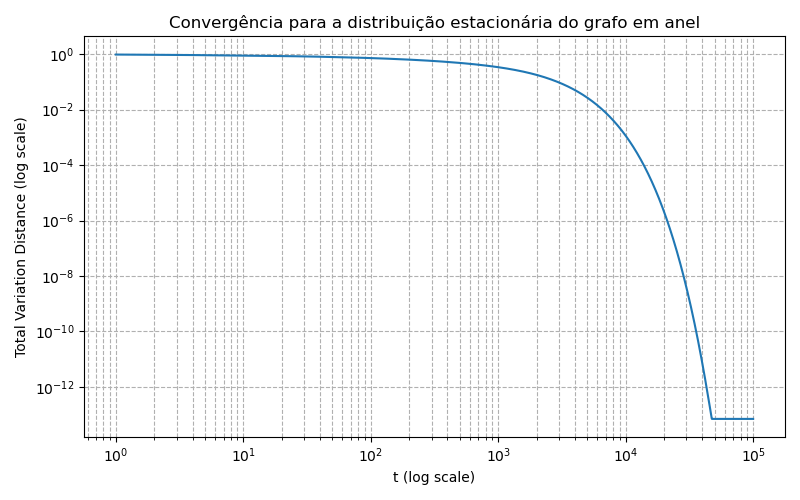
\includegraphics[width=0.75\textwidth]{fig/q2_anel.png}
            \item Grafo em árvore binária cheia ($n = 127$):
            
            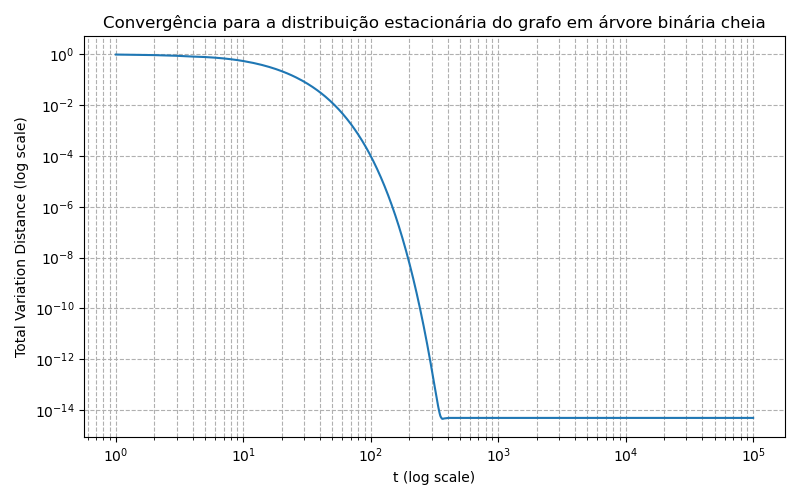
\includegraphics[width=0.75\textwidth]{fig/q2_arvore.png}
            \item Grafo em reticulado (grid) com duas dimensões ($n = 121$):
            
            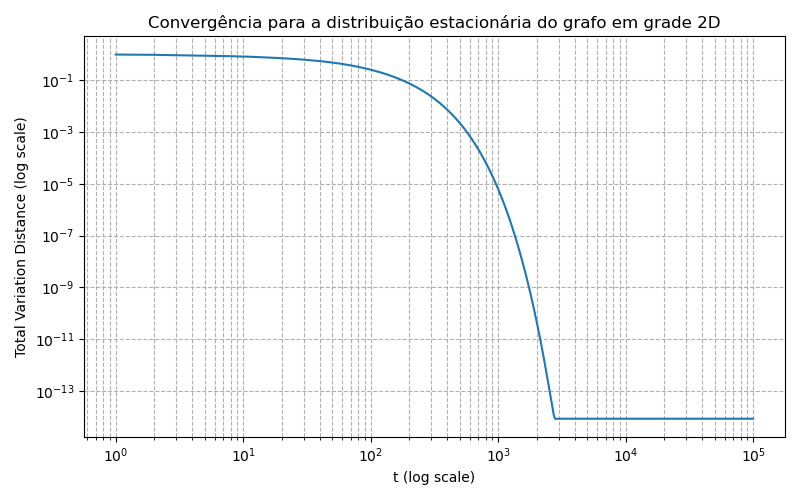
\includegraphics[width=0.75\textwidth]{fig/q2_grid.png}
        \end{itemize}
    \end{resposta}

    \item O que você pode concluir sobre a convergência em função da estrutura do grafo?
    \begin{resposta}
        O grafo em árvore binária cheia é o que apresenta convergência mais rápida, seguido pelo grafo em reticulado (grid) e, por último, o grafo em anel. Isso pode ser explicado pela estrutura de cada grafo: a árvore possui uma organização ramificada que permite ao passeio aleatório atingir diferentes regiões rapidamente. O reticulado também possui múltiplos caminhos entre os vértices, facilitando a dispersão da probabilidade ao longo do tempo. Já o grafo em anel, com conexões mais limitadas e estrutura cíclica, dificulta essa dispersão e, portanto, tende a convergir mais lentamente para a distribuição estacionária.
    \end{resposta}
\end{enumerate}

